%插入样式内容
\documentclass[12pt]{article}
%%---------------------------------------------------------------------
% packages
% geometry
\usepackage{geometry}
% font
\usepackage{fontspec}
\defaultfontfeatures{Mapping=tex-text}  %%如果没有它,会有一些 tex 特殊字符无法正常使用,比如连字符。
\usepackage{xunicode,xltxtra}
\usepackage[BoldFont,SlantFont,CJKnumber,CJKchecksingle]{xeCJK}  % \CJKnumber{12345}: 一万二千三百四十五
\usepackage{CJKfntef}  %%实现对汉字加点、下划线等。
\usepackage{pifont}  % \ding{}
% math
\usepackage{amsmath,amsfonts,amssymb}
% color
\usepackage{color}
\usepackage{xcolor}
\definecolor{EYE}{RGB}{199,237,204}
\definecolor{FLY}{RGB}{128,0,128}
\definecolor{ZHY}{RGB}{139,0,255}
% graphics
\usepackage[americaninductors,europeanresistors]{circuitikz}
\usepackage{tikz}
\usetikzlibrary{positioning,arrows,shadows,shapes,calc,mindmap,trees,backgrounds}  % placements=positioning
\usepackage{graphicx}  % \includegraphics[]{}
\usepackage{subfigure}  %%图形或表格并排排列
% table
\usepackage{colortbl,dcolumn}  %% 彩色表格
\usepackage{multirow}
\usepackage{multicol}
\usepackage{booktabs}
% code
\usepackage{fancyvrb}
\usepackage{listings}
% title
\usepackage{titlesec}
% head/foot
\usepackage{fancyhdr}
% ref
\usepackage{hyperref}
% pagecolor
\usepackage[pagecolor={EYE}]{pagecolor}
% tightly-packed lists
\usepackage{mdwlist}

\usepackage{styles/iplouccfg}
\usepackage{styles/zhfontcfg}
\usepackage{styles/iplouclistings}

\usepackage{color,framed}

%%---------------------------------------------------------------------
% settings
% geometry
\geometry{left=2cm,right=1cm,top=2cm,bottom=2cm}  %设置 上、左、下、右 页边距
\linespread{1.5} %行间距
% font
\setCJKmainfont{Adobe Kaiti Std}
%\setmainfont[BoldFont=Adobe Garamond Pro Bold]{Apple Garamond}  % 英文字体
%\setmainfont[BoldFont=Adobe Garamond Pro Bold,SmallCapsFont=Apple Garamond,SmallCapsFeatures={Scale=0.7}]{Apple Garamond}  %%苹果字体没有SmallCaps
\setCJKmonofont{Adobe Fangsong Std}
% graphics
\graphicspath{{figures/}}
\tikzset{
    % Define standard arrow tip
    >=stealth',
    % Define style for boxes
    punkt/.style={
           rectangle,
           rounded corners,
           draw=black, very thick,
           text width=6.5em,
           minimum height=2em,
           text centered},
    % Define arrow style
    pil/.style={
           ->,
           thick,
           shorten <=2pt,
           shorten >=2pt,},
    % Define style for FlyZhyBall
    FlyZhyBall/.style={
      circle,
      minimum size=6mm,
      inner sep=0.5pt,
      ball color=red!50!blue,
      text=white,},
    % Define style for FlyZhyRectangle
    FlyZhyRectangle/.style={
      rectangle,
      rounded corners,
      minimum size=6mm,
      ball color=red!50!blue,
      text=white,},
    % Define style for zhyfly
    zhyfly/.style={
      rectangle,
      rounded corners,
      minimum size=6mm,
      ball color=red!25!blue,
      text=white,},
    % Define style for new rectangle
    nrectangle/.style={
      rectangle,
      draw=#1!50,
      fill=#1!20,
      minimum size=5mm,
      inner sep=0.1pt,}
}
\ctikzset{
  bipoles/length=.8cm
}
% code
\lstnewenvironment{VHDLcode}[1][]{%
  \lstset{
    basicstyle=\footnotesize\ttfamily\color{black},%
    columns=flexible,%
    framexleftmargin=.7mm,frame=shadowbox,%
    rulesepcolor=\color{blue},%
%    frame=single,%
    backgroundcolor=\color{yellow!20},%
    xleftmargin=1.2\fboxsep,%
    xrightmargin=.7\fboxsep,%
    numbers=left,numberstyle=\tiny\color{blue},%
    numberblanklines=false,numbersep=7pt,%
    language=VHDL%
    }\lstset{#1}}{}
\lstnewenvironment{VHDLmiddle}[1][]{%
  \lstset{
    basicstyle=\scriptsize\ttfamily\color{black},%
    columns=flexible,%
    framexleftmargin=.7mm,frame=shadowbox,%
    rulesepcolor=\color{blue},%
%    frame=single,%
    backgroundcolor=\color{yellow!20},%
    xleftmargin=1.2\fboxsep,%
    xrightmargin=.7\fboxsep,%
    numbers=left,numberstyle=\tiny\color{blue},%
    numberblanklines=false,numbersep=7pt,%
    language=VHDL%
    }\lstset{#1}}{}
\lstnewenvironment{VHDLsmall}[1][]{%
  \lstset{
    basicstyle=\tiny\ttfamily\color{black},%
    columns=flexible,%
    framexleftmargin=.7mm,frame=shadowbox,%
    rulesepcolor=\color{blue},%
%    frame=single,%
    backgroundcolor=\color{yellow!20},%
    xleftmargin=1.2\fboxsep,%
    xrightmargin=.7\fboxsep,%
    numbers=left,numberstyle=\tiny\color{blue},%
    numberblanklines=false,numbersep=7pt,%
    language=VHDL%
    }\lstset{#1}}{}
% pdf
\hypersetup{%pdfpagemode=FullScreen,%
            pdfauthor={Haiyong Zheng},%
            pdftitle={Title},%
            CJKbookmarks=true,%
            bookmarksnumbered=true,%
            bookmarksopen=false,%
            plainpages=false,%
            colorlinks=true,%
            citecolor=green,%
            filecolor=magenta,%
            linkcolor=cyan,%red(default)
            urlcolor=cyan}
% section
%http://tex.stackexchange.com/questions/34288/how-to-place-a-shaded-box-around-a-section-label-and-name
\newcommand\titlebar{%
\tikz[baseline,trim left=3.1cm,trim right=3cm] {
    \fill [cyan!25] (2.5cm,-1ex) rectangle (\textwidth+3.1cm,2.5ex);
    \node [
        fill=cyan!60!white,
        anchor= base east,
        rounded rectangle,
        minimum height=3.5ex] at (3cm,0) {
        \textbf{\thesection.}
    };
}%
}
\titleformat{\section}{\Large\bf\color{blue}}{\titlebar}{0.1cm}{}
% head/foot
\setlength{\headheight}{15pt}
\pagestyle{fancy}
\fancyhf{}

\chead{\color{black!50!green}DIGITS DevBox}

%\lfoot{\color{blue!50!green}Dai Jialun}
\cfoot{\color{blue!50!green}\href{http://vision.ouc.edu.cn/~zhenghaiyong}{CVBIOUC}}
\rfoot{\color{blue!50!green}$\cdot$\ \thepage\ $\cdot$}
\renewcommand{\headrulewidth}{0.4pt}
\renewcommand{\footrulewidth}{0.4pt}


%%---------------------------------------------------------------------
\begin{document}
%%---------------------------------------------------------------------
%%---------------------------------------------------------------------
% \titlepage
\title{\vspace{-2em} DIGITS DevBox深度学习服务器\\
\normalsize{}}
\author{Dai Jialun}
\date{\vspace{-0.7em} \today \vspace{-0.7em}}
%%---------------------------------------------------------------------
\maketitle\thispagestyle{fancy}
%%---------------------------------------------------------------------
\maketitle
%\tableofcontents 
\section{硬件配置}
实验室所组装的DIGITS DevBox深度学习服务器,以下是其具体硬件配置。这台服务器的原型为NVIDIA官方生产的\href{https://developer.nvidia.com/devbox}{DIGITS DevBox},可参考其配置。
\begin{description}
\item[显卡] 4个ASUS(华硕)GTX 980Ti-6GD5
\definecolor{shadecolor}{rgb}{0.92,0.92,0.92}  
\begin{shaded}
\scriptsize{
芯片厂商: NVIDIA

显卡芯片: GeForce GTX 980Ti

显示芯片系列: NVIDIA GTX 900系列

核心代号: GM200

显存类型: GDDR5

显存容量: 6144MB

显存位宽: 384bit

最大分辨率: 4096×2160

接口类型: PCI Express 3.0 16X

I/O接口: HDMI接口/DVI接口/3个DisplayPort接口

电源接口: 8pin+6pin

产品尺寸:266.7×111.2×38.1mm

参考报价:5999*4=23996} 
\end{shaded}   
\item[CPU] 1个Intel(英特尔) Core i7-5960X
\definecolor{shadecolor}{rgb}{0.92,0.92,0.92}  
\begin{shaded}
\scriptsize{
CPU主频:3GHz

最高睿频:3.5GHz 

总线类型:QPI总线

总线频率:8GT/s

插槽:LGA 2011-v3 

CPU架构:Haswell

核心:八核心十六线程

制作工艺: 22纳米

功耗: 140W

三级缓存: 20MB

最大支持内存:64G

指令集:SSE4.2,AVX 2.0,AES

内存控制器:四通道:DDR4 1333/1600/2133

参考报价: 7699 RMB} 
\end{shaded}   
\item[主板] 1个ASUS(华硕)X99-E WS
\definecolor{shadecolor}{rgb}{0.92,0.92,0.92}  
\begin{shaded}
\scriptsize{
主芯片组:Intel X99

CPU插槽:LGA 2011-3

支持CPU数量: 1颗

内存类型: DDR4

内存插槽: 8*DDR4 DIMM

最大内存容量: 128GB

内存描述:支持四通道DDR4 3000(超频)/3200(O.C.)/2800(超频)/2666(超频)/2400(超频)/2133MHz内存

显卡插槽: PCI-E 3.0标准

PCI-E插槽:7×PCI-E X16显卡插槽

SATA接口: 8×SATA III接口;1×SATA Express接口;1×M.2接口(10Gb/s)

USB接口: 12×USB3.0接口(10背板+2内置);4×USB2.0接口(2背板+2内置)

版型:E-ATX板型

外形尺寸:30.5×26.7cm 

多显卡技术:支持NVIDIA 4-Way SLI四路交火技术

RAID功能:支持RAID 0,1,5,10 

尺寸:30.5 厘米 x 26.7 厘米

参考报价: 4799 RMB} 
\end{shaded}   
\item[内存] 2个CORSAIR(海盗船) VENGERNCE(复仇者)LPX 32GB(4 $\times$ 8GB) DDR4 2400MHz CMK32GX4M4A2400C14R
\definecolor{shadecolor}{rgb}{0.92,0.92,0.92}  
\begin{shaded}
\scriptsize{
内存容量:套装(4×8GB)

内存类型:DDR4

内存主频:2400MHz

参考报价:5000*2=10000 RMB} 
\end{shaded} 
\item[硬盘] 3个WesternDigital(西部数码) 4TB 7200转
\definecolor{shadecolor}{rgb}{0.92,0.92,0.92}  
\begin{shaded}
\scriptsize{
硬盘容量:4000G

缓存:64M

转速:7200rpm

接口类型:SATA3.0

接口速率:6Gb/s

参考报机:1799*3=5397 RMB} 
\end{shaded} 
\item[固态硬盘] 1个Samsung(三星)SSD 850pro 512GB
\definecolor{shadecolor}{rgb}{0.92,0.92,0.92}  
\begin{shaded}
\scriptsize{
接口类型:SATA3

硬盘尺寸:2.5英寸

参考报价:2999 RMB} 
\end{shaded} 
\item[固态硬盘] 1个Samsung SSD 512GB SM951 cache for RAID
\definecolor{shadecolor}{rgb}{0.92,0.92,0.92}  
\begin{shaded}
\scriptsize{
参考报价:3450 RMB} 
\end{shaded} 
\item[机箱] 1个CORSAIR(海盗船) 900D
\begin{shaded}
\scriptsize{
机箱样式:台式机箱(全塔)

适用主板:**EATX板型**,ATX板型,MATX板型

电源类型:标准ATX PS2电源(选配)

电源设计:下置电源

显卡限长:400mm

5.25英寸仓位:4个

3.5英寸仓位:9个

2.5英寸仓位:9个

扩展插槽:10

前置接口:4*USB 2.0;2*USB 3.0

散热性能:前:3×120mm风扇(标配),
   	顶:4×120mm或3*140mm风扇(选配),
        后:1×140mm风扇(标配),
        底:8×120mm或6*140mm风扇(选配)

尺寸:649.6×252×691.6mm

参考报价:2499 RMB } 
\end{shaded} 
\item[电源] 1个CORSAIR(海盗船) AX1500i 1500W
\definecolor{shadecolor}{rgb}{0.92,0.92,0.92}  
\begin{shaded}
\scriptsize{
功率:1500W

风扇描述:14cm风扇

电源尺寸:150x86x225mm

参考报价:3599 RMB} 
\end{shaded} 
\item[散热器] 1个CORSAIR(海盗船) H110 水冷CPU散热器
\definecolor{shadecolor}{rgb}{0.92,0.92,0.92} 
\begin{shaded}
\scriptsize{
参考报价:999 RMB} 
\end{shaded} 
\item[风扇] 6个CORSAIR(海盗船)AF120 静音版 双包装
\definecolor{shadecolor}{rgb}{0.92,0.92,0.92} 
\begin{shaded}
\scriptsize{
参考报价:89*12=1068 RMB} 
\end{shaded} 
\item[光驱] 1个AUSU(华硕)DRW-24D1ST
\definecolor{shadecolor}{rgb}{0.92,0.92,0.92} 
\begin{shaded}
\scriptsize{
参考报价:120 RMB} 
\end{shaded} 
\item[配件] 1个Thermaltake Commander FT触控式面板风扇控制器,Deepcool FAN HUB(九州风神风扇集线器)
\definecolor{shadecolor}{rgb}{0.92,0.92,0.92} 
\begin{shaded}
\scriptsize{
参考报价:299 RMB} 
\end{shaded} 
\item[显示器]
\item[键盘鼠标]
\end{description}

\section{名词解释}
\begin{description}

\item[DVI] Digital Visual Interface,数字视频接口
\begin{figure}[!h]
\centering
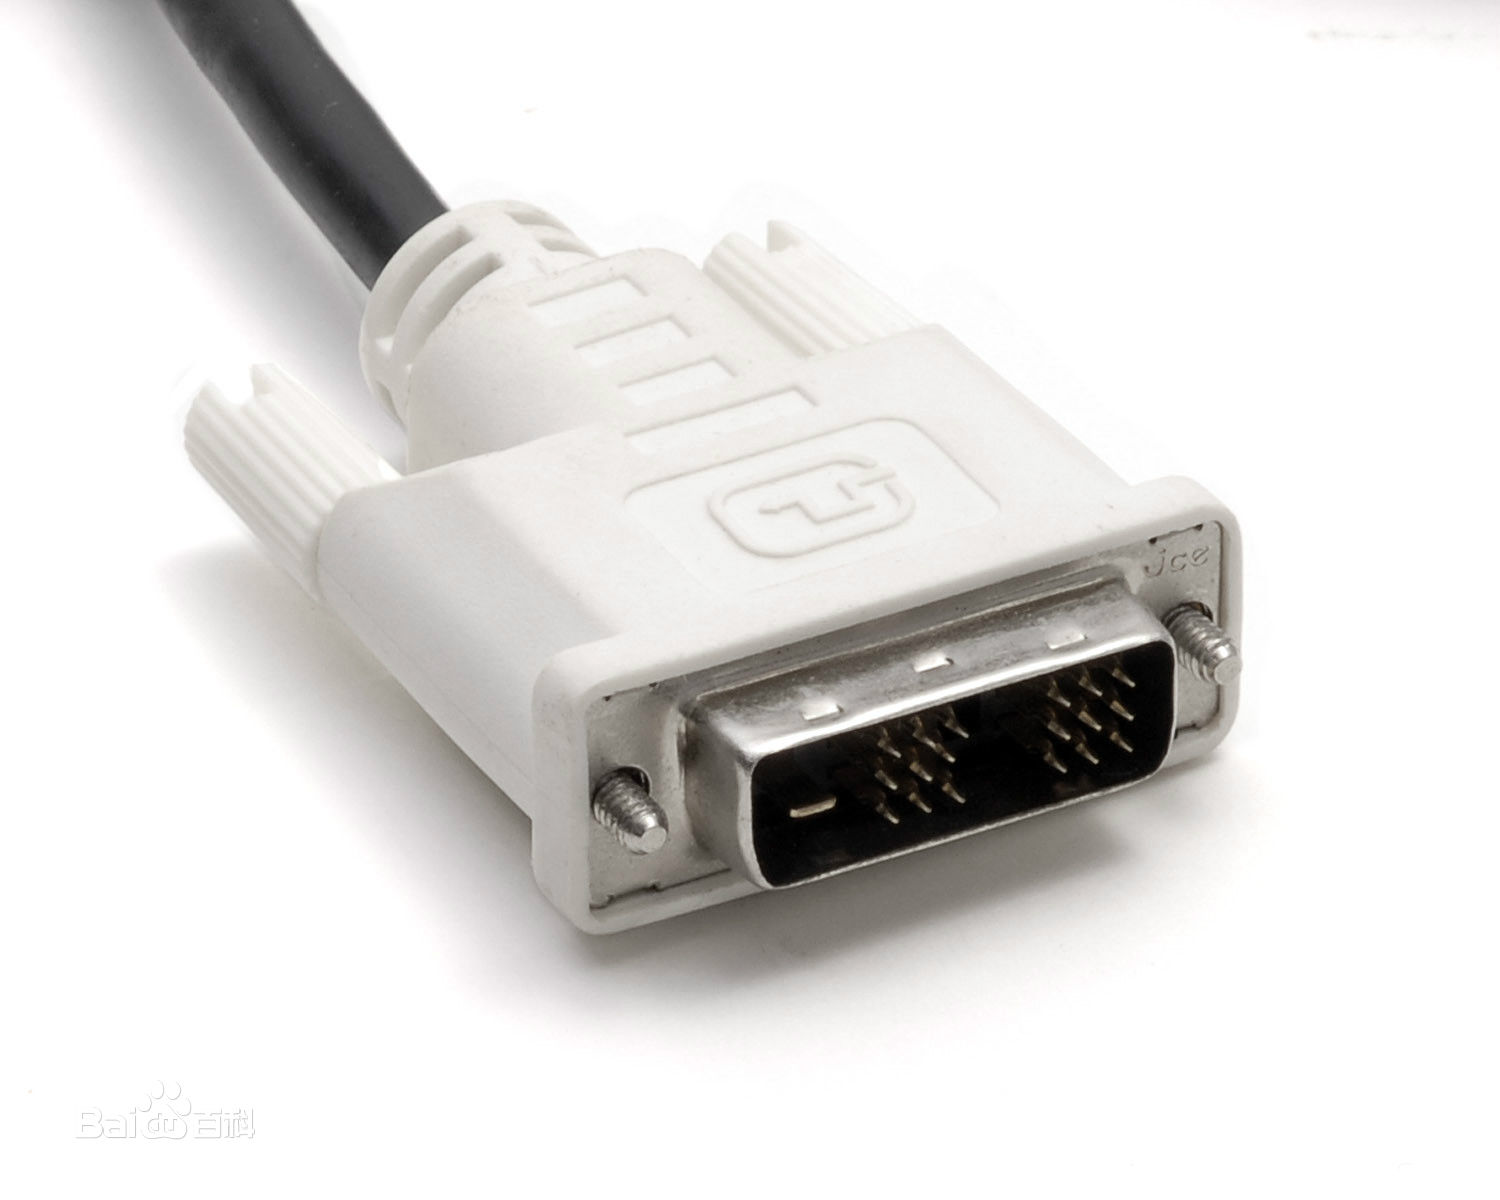
\includegraphics[width=0.2\textwidth]{DVI}
\end{figure}

\item[DislayPort] 高清数字显示借口标准
\begin{figure}[!ht]
\centering
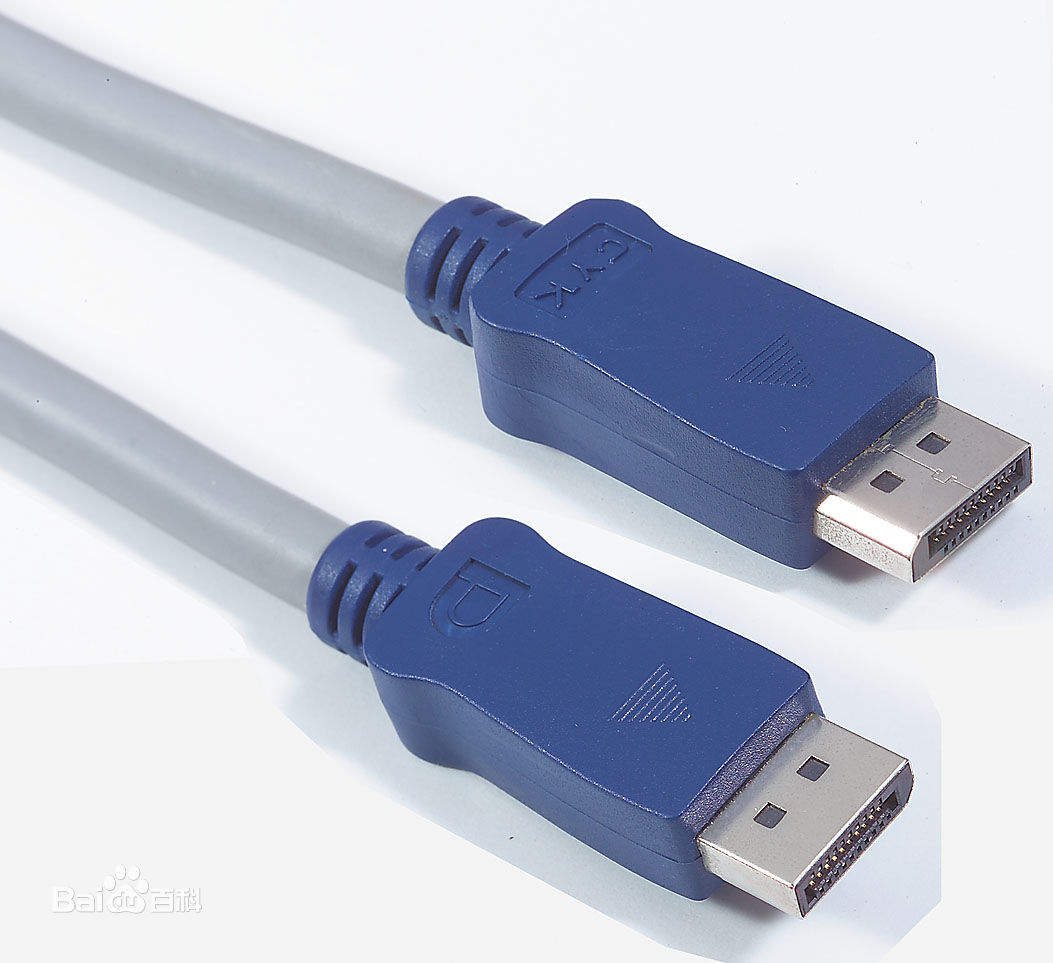
\includegraphics[width=0.2\textwidth]{DisplayPort}
\end{figure}

\item[PCI-E] PCI Express,新的总线接口
\begin{figure}[!ht]
\centering
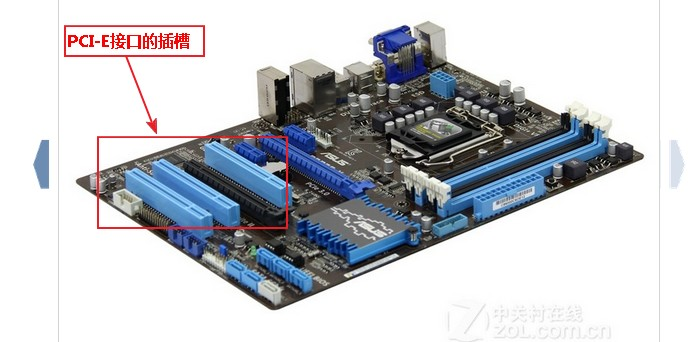
\includegraphics[width=0.2\textwidth]{PCI-E}
\end{figure}

\item[SATA Revision 3.0] Serial Advanced Technology Attachment,串行ATA规格第三版,6Gbps
\begin{figure}[!ht]
\centering
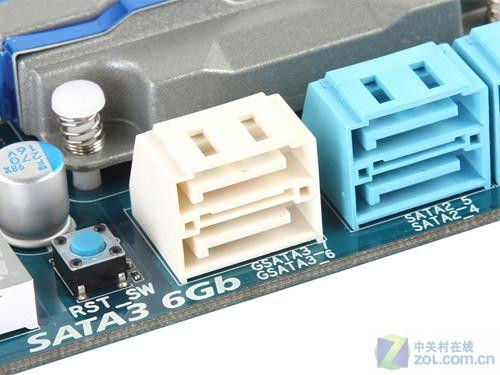
\includegraphics[width=0.2\textwidth]{SATA3}
\end{figure}

\item[SATA EXpress] SATA 3.0下一代的SATA接口,10Gbps
\begin{figure}[!ht]
\centering
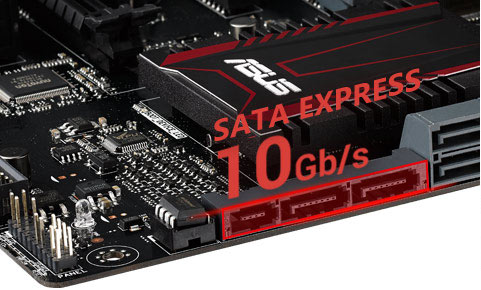
\includegraphics[width=0.2\textwidth]{SATAE}
\end{figure}

\item[M.2] 一种替代MSATA新的接口规范,优势体现在速度和体积。支持Socket2和Socket3两种接口类型
\begin{figure}[!ht]
  \centering 
  \subfigure[]{ 
    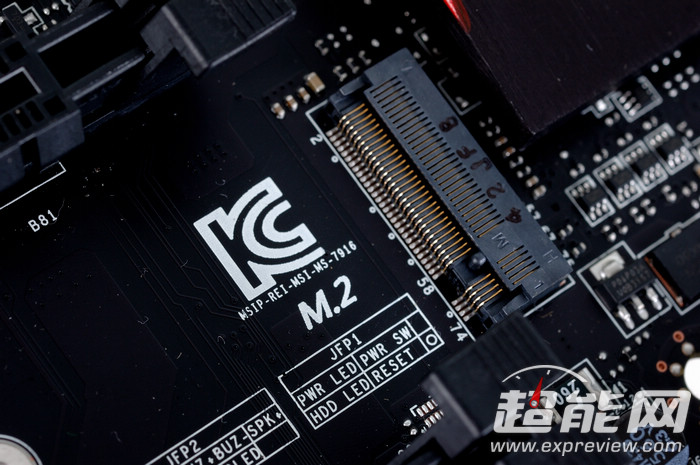
\includegraphics[width=0.23\textwidth]{M2}} 
  \subfigure[]{ 
    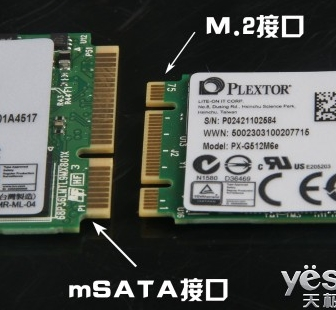
\includegraphics[width=0.17\textwidth]{M2-MSATA}} 
  \caption{}
\end{figure}

\item[RAID] Redundant Arrays of Independent Disks,磁盘阵列。磁盘阵列是由很多价格较便宜的磁盘,组合成一个容量巨大的磁盘组,利用个别磁盘提供数据所产生加成效果提升整个磁盘系统效能。利用这项技术,将数据切割成许多区段,分别存放在各个硬盘上。
\begin{figure}[!ht]
  \centering 
  \subfigure[]{ 
    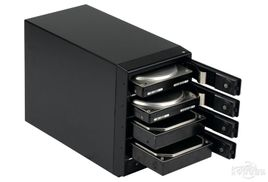
\includegraphics[width=0.24\textwidth]{RAID1}} 
  \subfigure[]{ 
    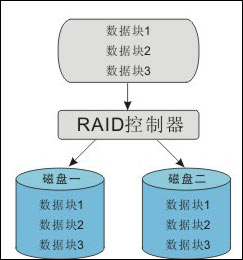
\includegraphics[width=0.15\textwidth]{RAID2}} 
  \caption{}
\end{figure}

\item[RAID5] 一种存储性能、数据安全和存储成本兼顾的存储解决方案。为系统提供数据安全保障,但保障程度要比Mirror低而磁盘空间利用率要比Mirror高。数据以块为单位分布到各个硬盘上。RAID 5不对数据进行备份,而是把数据和与其相对应的奇偶校验信息存储到组成RAID5的各个磁盘上,并且奇偶校验信息和相对应的数据分别存储于不同的磁盘上。当RAID5的一个磁盘数据损坏后,利用剩下的数据和相应的奇偶校验信息去恢复被损坏的数据。
\begin{figure}[!ht]
\centering
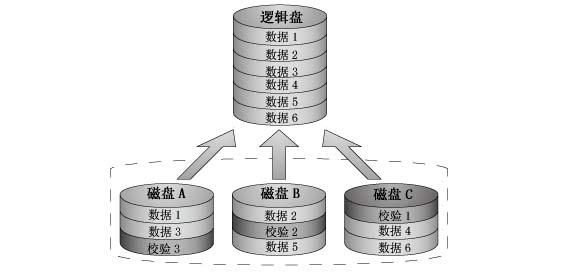
\includegraphics[width=0.4\textwidth]{RAID5}
\end{figure}

\item[SLI] Scalable Link Interface,可灵活伸缩的连接接口(支持多显卡技术)。这是一种可把两张或以上的显卡连在一起,作单一输出使用的技术,从而达至绘图处理效能加强的效果。
\begin{figure}[!ht]
\centering
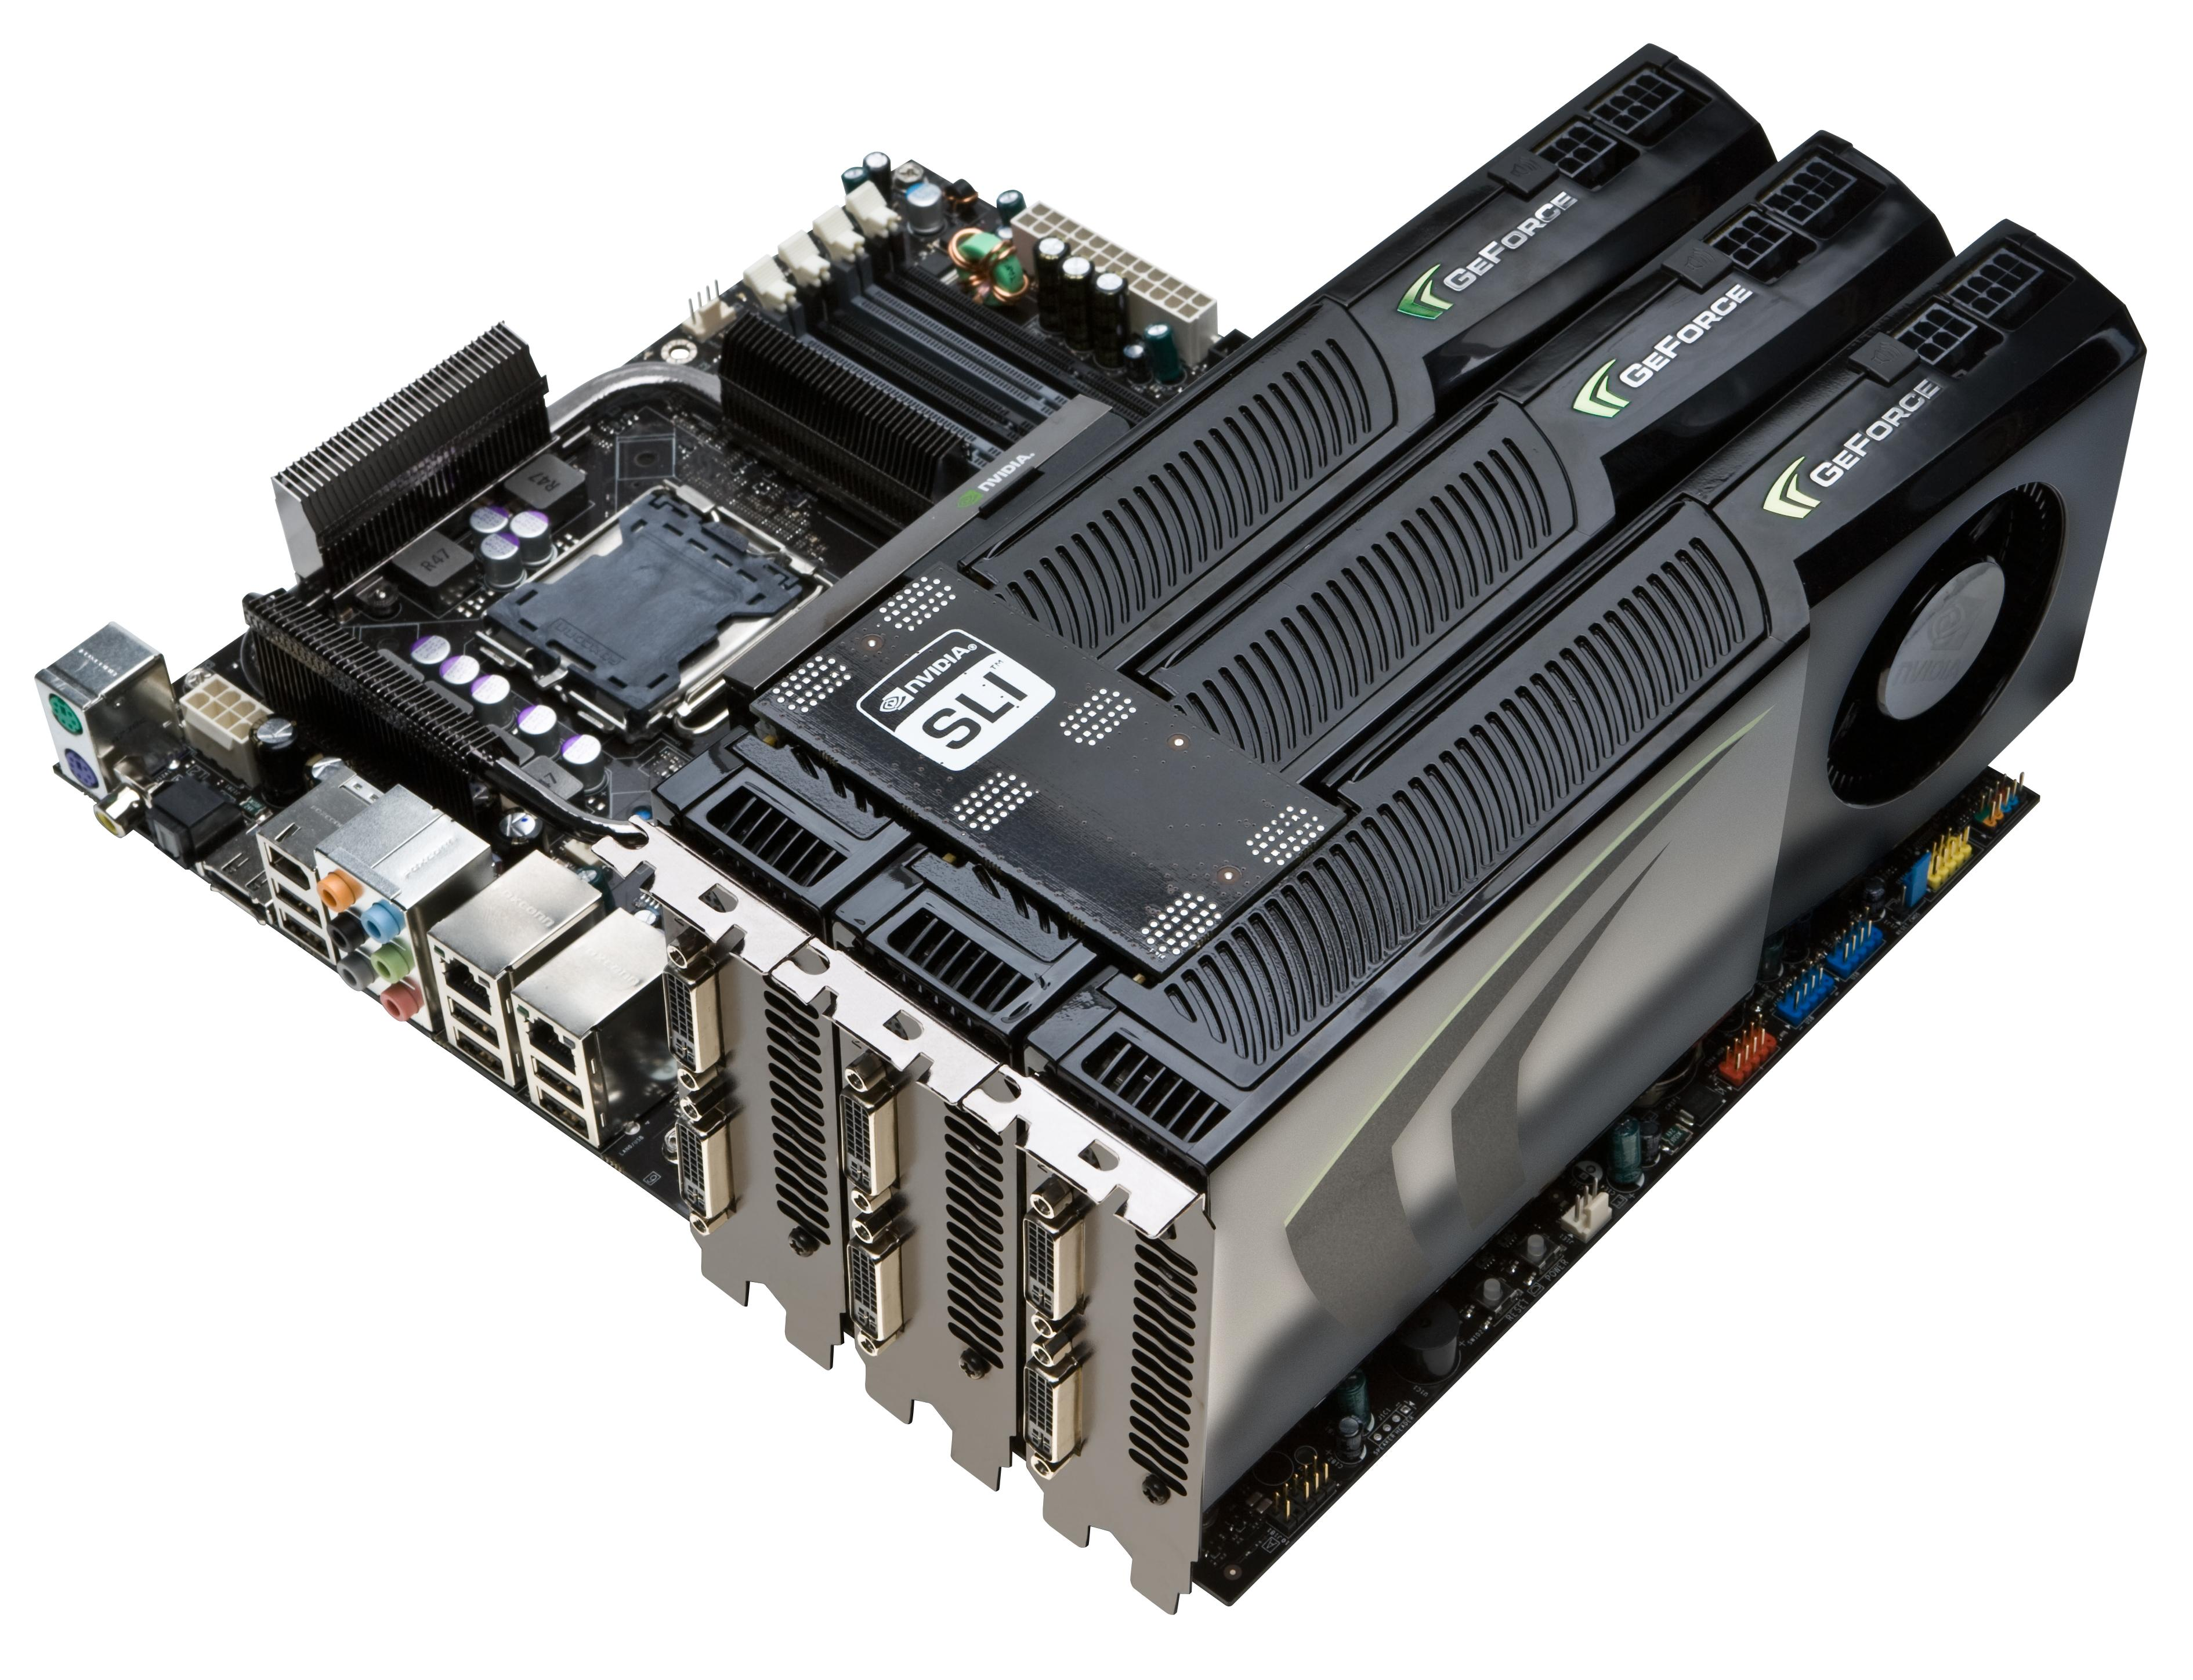
\includegraphics[width=0.2\textwidth]{SLI}
\end{figure}

\item[DDR4] Dual Data Rate SDRAM,是一种高速CMOS动态随即访问的内存。DDR4支持2133MHz,32GB DDR4-2133达到48.4GB/s。

\item[GDDR5] Graphics Double Data Rate SDRAM version5,是一种高性能显卡用内存,需搭配支持PCI-E以上规格的显卡,高频率达4GHZ,低功耗。

\item[UEFI] Unified Extensible Firmware Interface,统一的可扩展固件接口,是一种详细描述类型接口的标准。这种接口用于操作系统自动从预启动的操作环境,加载到一种操作系统上。
\item[BIOS] Basic Input/Output System,基本输入/输出系统。
\item[固件] Firmware,固定软件(自己理解),写入EROM或EEPROM中的程序。固件担任着一个系统最基础最底层工作的软件。初期,这些硬件内所保存的程序是无法被用户直接读出或修改的,如今这些是可以重复刷写的,让固件得以修改和升级。
\item[MRB分区] MRB分区表是将磁盘的分区信息保存到磁盘的第一个扇区(MRB扇区)的64个字节中,每个分区项(文件系统、起始柱面号、磁头号等信息)占有16个字节,因此总共只能记录4个主分区,由于在一个分区项中用4个字节存储分区的总扇区数($2^{32}$),每扇区512字节($2^{9}B$),因此每个分区不能超过2TB($2^{32} \times 2^{9}B=2^{41}B=2TB$)。磁盘容量超过2TB以后,分区的起始位置也就无法表示了。
\item[GPT分区] GPT分区表是基于可扩展固件借口(EFI)使用的磁盘分区架构,支持每个磁盘可达到128个分区,且最大容量可达18EB。
\item[cuDNN] CUDA Deep Neural Network library\footnote{http://devblogs.nvidia.com/parallelforall/accelerate-machine-learning-cudnn-deep-neural-network-library/},是专门针对Deep Learning框架设计的一套GPU计算加速方案,使工作者投入与设计和训练神经网络模型,而不用在底层的表现上话费时间。目前支持的DL工具包括caffe,Theano和Torch等。cuDNN的Realease版本有cuDNN v1,cuDNN v2 for CUDA 6.5 and later 和cuDNN v3 for CUDA 7.0 and later.
\item[CUDA] Compute Unified Device Architecture,是一种由NVIDIA推出的通用并行计算架构,该架构使GPU能够解决商业、工业以及科学方面的复杂计算问题。在架构上采用了一种全新的计算体系结构来使用GPU提供的硬件资源,从而给大规模的数据计算应用提供了一种比CPU更加强大的计算能力,即将显卡中的充分使用GPU来解决大量数据计算问题。开发人员可使用C语言来为CUDA架构编写程序,所编写出的程序可在支持CUDA的处理器上以超高性能运行。CUDA3.0已经开始支持C++和FORTRAN。
\item[CUDA Toolkit] CUDA Toolkit是进行CUDA开发所需要的一个软件。它通过GPU加速技术,给C和C++开发者提供了一个综合的开发环境。CUDA Toolkit包括NVIDIA GPUs编译器,数学库以及debug和优化。
\item[HDF] Hierarchical Data Format,可以存储不同类型的图像和数码数据的文件格式,并且可以在不同类型的机器上传输,同时还有统一处理这种文件格式的函数库。大多数普通计算机都支持这种文件格式。文件格式是指计算机存储和处理数据的方式 。目前常用的图像文件格式很多, 如 GIF、JPG等 ,其共同的缺点是结构太简单 ,不能存放除影像信息外其他的有用数据 ,像遥感影像的坐标值、参数等都无法保存,而且用不同格式存储影像数据使得读取、传输、共享变得复杂, 因此,有必要建立一种标准格式以解决上述问题。
\item[HDF5] HDF5能处理更多的对象 ,存储更大的文件 ,支持并行 I/O ,线程和具备现代操作系统与应用程序所要求的其他特性, 而且数据模型变得更简单 ,概括性更强。HDF5 只有两种基本结构 :组(group)和数据集(dataset)。
\item[DIGITS] NVIDIA Deep Learning GPU Training System,通过对数据实行可视化的实时检测,让开发者快速设计出深度神经网络。DIGITS最大的特点是,你不需要写任何的代码就可快速上手DIGITS。DIGITS是通过网络浏览器来进入的网页应用。
\end{description}



\section{RAID5}
\subsection{RAID的优点}
\begin{itemize}
\item 可高效恢复磁盘
\item 增强了速度
\item 扩容了存储能力
\end{itemize}

\subsection{实现RAID方法}
\begin{description}
\item[硬RAID] Hardware RAID,通过用硬件(RAID卡或者磁盘阵列)来实现RAID功能。硬件RAID具备了自身的RAID控制/处理与I/O处理芯片,甚至还有阵列缓冲(Array Buffer),对CPU的占用率以及整体性能都是最优势的,但设备成本也是三最高的。Hardware RAID自成一个单元,由自身硬件和软件管理RAID,与主板和操作系统无关,即Ubuntu不需要额外的程序来管理。
\item[软RAID] Software RAID,通过用操作系统的软件程序(Linux系统下的mdadm命令)来完成RAID功能。软件RAID的所有功能都是操作系统与CPU 来完成,没有第三方的控制/处理与I/O 芯片,与主板BIOS程序无关,其效率与稳定性较低。例如在Ubuntu系统下的软RAID,其格式化、挂载、写入与重建全部由mdadm负责。
\item[伪RAID] Fake RAID,又称BIOS RAID。通过主板的集成芯片,内建RAID控制器来创建阵列,由操作系统驱动识别(主要表现在Intel Desktop的主板上表现的比较明显)。由于缺乏独立的I/O处理芯片,所以这方面的工作仍要由CPU与驱动程序来完成。另外,Fake RAID所采用的RAID控制/处理芯片的能力一般都比较弱,不能支持高的RAID等级。在Intel集成芯片的主板,主要使用Intel Rapid Storage Technology来管理,该技术主要支持Window系统,不支持Linux系统。在Linux系统下,Intel主要使用dmraid和mdadm来管理RAID,推荐使用mdadm。
\end{description}

\subsection{主板集成RAID与外插RAID卡区别}
\begin{description}
\item[性能] 主板集成的RAID,它的性能以及速度是通过主板的CPU与内存来实现的,它会占有主板一定的带宽,会影响整机的性能;外插RAID卡,有自己的CPU和内存,所以数据处理大部分都会独立处理,不会影响主板上的CPU与内存速度。总体看来,外插的RAID卡的RAID要比主板集成的RAID快得多。
\item[安全性] 主板集成的RAID,其安全性不能够得到保证,因为是通过更改主板的BIOS选项做成的,所以一旦主板损坏、主板的CMOS电池掉电或无意更改了主板BIOS的设置都会带来RAID的丢失。通过主板做成的RAID,一旦丢失,将会不能恢复,后果是非常严重的;而外插的RAID卡所做成的RAID,不会因为主板损坏、主板的CMOS电池掉电等现象对数据造成影响,所以外插的RAID卡,其安全性远远大于主板集成的。另外,Raid完全由Ubuntu的mdadm命令管理。
\end{description}


\subsection{实现RAID方法比较}
在这台DIGITS DevBox的RAID主要是Fake RAID和Software RAID,对别对应的软件是dmraid和mdadm。Intel同时支持dmraid和mdadm,但是更推荐使用mdadm。
\subsubsection{dmraid}
\begin{itemize}
\item dmraid主要是属于Fake RAID来创建、管理RAIDd的。在启动时候,由主板上的芯片驱动RAID,当载入Linux内核之后,由Linux接手管理,消耗cpu和内存等资源\footnote{http://www.cnblogs.com/linuxer/archive/2012/03/07/2441224.html}。在Ubuntu系统中,dmraid主要是将硬件的RAID映射成系统中/dev/mapper/目录下的设备,例如/dev/mapper/isw\_dfadcda\_Volume1,其中isw为intel的硬件名字,Volume1为RAID名称\footnote{http://book.51cto.com/art/200902/110754.htm}。
\item 在BIOS创建的RAID,在Ubuntu系统中,可能会出现大容量硬盘识别不正确的问题。例如,在BIOS中创建的3 个3.6TB的硬盘组成的RAID5,理论上应该为7.2TB,但是Ubuntu系统只能识别为3.6TB,容量偏小,而Ubuntu Server和Debian甚至都无法识别,不显示。
\item 不推荐使用dmraid命令。首先,dmraid从2011年已经不提供更新了,而mdadm仍然不测试和更新;其实,dmraid对于大容量硬盘的识别容易出错,如今的硬盘都是1TB以上的,对于dmraid很容易造成错误;最后,dmraid是将RAID映射成mapper,无法真正实现RAID数据恢复等高级功能。
\end{itemize}

\subsubsection{mdadm}
\begin{itemize}
\item 在linux系统中目前以MD(Multiple Devices)虚拟块设备的方式实现软件RAID,利用多个底层的块设备虚拟出一个新的虚拟设备,即使用mdadm命令\footnote{http://blog.csdn.net/yuesichiu/article/details/8502680}。
\item Fake RAID只提供廉价的控制器,RAID处理开销仍由CPU和内存负责,因此性能与效率基本与Software RAID基本一直。对于Linux系统,使用Software RAID一般比Fake RAID更稳定和安全\footnote{http://blog.163.com/jiangh\_1982/blog/static/12195052014252131760/}。
\item Ubuntu的软RAID相关命令为mdadm,其配置、测试、删除参考\footnote{http://blog.itpub.net/27771627/viewspace-1246416/}。 
\item \textbf{在没有Hardware RAID的条件下,推荐使用mdadm实现RAID}。
\end{itemize}


\subsection{创建RAID5步骤(Ubuntu下Software RAID,推荐!!!)}
在Ubuntu系统中,通常使用mdadm,即Software RAID方法来创建RAID5\footnote{http://blog.itpub.net/27771627/viewspace-1246416/}
\begin{enumerate}
\item \textbf{安装mdadm,查看实际磁盘情况}。
\begin{bash}
sudo apt-get install mdadm
sudo fdisk -l
\end{bash}
\item \textbf{初始化}。。对各个磁盘删除分区(fdisk命令),且进行格式化(mkfs命令)。小容量硬盘(不到2TB)使用MRB分区表,大容量硬盘(2TB以上)使用GPT分区\footnote{http://wangheng.org/shi-yong-parted-chuang-jian-gpt-fen-qu.html}。
\begin{bash}
sudo fdisk -l		   #查看磁盘空间以及分区
sudo fdisk /dev/sdX  #用fdisk对某块硬盘处理,/dev/sdX中X表示磁盘号,例如/dev/sdb
sudo mkfs.ext4 /dev/sdX    #用mkfs将/dev/sdX格式化为ext4格式
sudo parted /dev/sdX	#用parted工具对大容量硬盘分区,为GPT分区
\end{bash}
\item \textbf{创建RAID5}
\begin{bash}
sudo fdisk -l		   #查看磁盘空间以及分区
sudo fdisk /dev/sdX  #用fdisk对某块硬盘处理,/dev/sdX中X表示磁盘号,例如/dev/sdb
sudo mdadm -C /dev/md0 -l5 -n3 /dev/sdb1 /dev/sdb /dev/sdc /dev/sdd   #sdb,sdc和sdd为磁盘,md0为创建好的RAID盘
sudo parted /dev/sdX	#用parted工具对大容量硬盘分区,为GPT分区
\end{bash}
\item \textbf{格式化}
\begin{bash}
cat /proc/mdstat	#查看RAID恢复进度
sudo mdadm -D /dev/md0  #查看RAID详细情况
\end{bash} 
\item \textbf{挂载}
\begin{bash}
sudo mkdir /deep		#在/目录下创建/deep
sudo mount /dev/md0 /deep  	#将md0挂载到/deep下
\end{bash} 
\item \textbf{自动挂载}。将/dev/md0 /deep ext4 defaults 1 2,写入/etc/fstab。建议重启后再查看RAID的磁盘号,可能我们创建的盘号为md0,但是重启后显示为md127,如果将之前的/dev/md0直接写入/etc/fstab,如果出错,可能导致重启出现问题。
\begin{bash}
sudo vim /etc/fstab 
\end{bash}
\end{enumerate}


\section{Caffe}
\subsection{Caffe配置}
\textbf{在本台DIGITS DevBox中,Caffe所安装的依赖或者库文件:}
\begin{itemize}
\item Ubuntu 14.04.3(默认情况为Ubuntu 14.04.3,暂时不推荐使用15.04)
\item 显卡驱动346.82(最新版为355.06)
\item CUDA7.0
\item cuDNN v2(cuDNN v3已更新)
\item OpenCV3.0.0rc1(推荐用这个包,之前下载的库在安装事可能出现问题)
\item Python 2.7.6(自动安装)
\item Matlab2014b
\item MKL(作为BLAS,使用parallel\_studio\_xe\_2015\_update2.tar.gz,目前2016版已更新)
\item glog(Google Logging Library,glog-0.3.3)
\end{itemize}
NVIDIA的DIGITS DevBox\href{http://docs.nvidia.com/deeplearning/digits-devbox-sw-release-notes/index.html#axzz3k5SLx3Q7}{默认软件配置},可作参考。

\subsection{Caffe安装}
目前,Caffe主要的安装步骤是参考了欧新宇老师博客中的\href{http://ouxinyu.github.io/Blogs/20140723001.html}{Caffe + Ubuntu 15.04 + CUDA 7.0 新手安装配置指南}。安装Caffe时请认真阅读。

\subsection{问题解决}
\begin{itemize}
\item 在安装过程中,必须根据CUDA版本选择NVIDIA驱动版本,例如CUDA7.0对应的版本应该是NVIDIA346版。如果按照Caffe安装步骤给出的方法,基本上不会出现问题。但是如果是手动安装NVIDIA驱动,且安装了最新版本驱动,例如安装了最新的355版本后,可能显示{\color{blue}{no CUDA-capable device is detected}}。则卸载最新版本保证回到对应版本驱动。
\begin{bash}
sudo ./NVIDIA-Linux-x86_64-355.06.run --unisntall
\end{bash}
\item 目前(2015.08.26)的从caffe的Github上下载的caffe-master是有问题的,因为很多文件格式改为了*.h5,这是HDF5格式。没有依赖文件的话,Ubuntu暂时不支持。如果碰到如果问题,将*.h5格式全去掉.h5,改为二进制格式则正常运行。例如在caffer-master/examples/cifar10/train\_quick.sh,caffer-master/examples/cifar10/train\_quick.sh与caffer-master/examples/imagenet/train\_caffenet.sh。目前该问题只能通过这个方法解决,但是在将来可以查看、安装\href{https://github.com/live-clones/hdf5}{HDF5}来尝试解决问题。
\item 在Github的Caffe库里的release版本存在很多错误,例如caffe-rc2,或许是编译或者安装问题,总之尽量使用最新的或者服务器上的Caffe版本。
\end{itemize}

\section{DIGITS}
\href{http://devblogs.nvidia.com/parallelforall/digits-deep-learning-gpu-training-system/}{DIGITS}是一款检测深度学习的软件工具。目前使用的版本为DIGITS v2.0.0-rc for Ubuntu 14.04
\subsection{软件需求}
\begin{itemize}
\item NVIDIA驱动版本必须是346或者更高版本
\item CUDA toolkit(>=6.5)
\item cuDNN
\item Caffe或Torch
\item graphviz
\begin{bash}
sudo apt-get install graphviz
\end{bash}
\end{itemize}

\subsection{安装GIGITS}
\begin{enumerate}
\item 下载安装包\href{https://developer.nvidia.com/digits}{digits-2.0.0-rc.tar.gz}
\item 解压安装包
\begin{bash}
tar xvf digits-2.0.0-rc.tar.gz
\end{bash}
\item 进入解压目录digits-2.0,运行安装脚本
\begin{bash}
cd digits-2.0
./install.sh
\end{bash}
\item 运行runme.sh,启动DIGITS server。在浏览器打开http://localhost:5000/来查看DIGITS工具。
\begin{bash}
./runme.sh
\end{bash}
\end{enumerate}

\subsection{DIGITS使用}
DIGIST主要是通过浏览器的网页应用。具体操作可参考\href{http://devblogs.nvidia.com/parallelforall/digits-deep-learning-gpu-training-system/}{官网}。



\section{其他工作}
\subsection{安装NVIDIA显卡驱动}
\textbf{此方法只适合安装NVIDIA最新的显卡驱动,较为麻烦,不推荐使用,只供参考。在Caffe安装过程中,提供了更简便的方法来安装NVIDIA显卡驱动,请使用其方法。}
\begin{enumerate}
\item 以下是驱动来源,更新受限制驱动列表(源)。
\begin{itemize}
\item 开源驱动nouveau(livecd安装时用的驱动)
\item 源(受限制驱动列表)
\item PPA源(一般是私人建的,方便群众用)
\item 自己下载编译的驱动(我们使用的方法)
\end{itemize}
\begin{bash}
sudo apt-get install nvidia-current nvidia-settings
\end{bash}
\item 下载驱动
	\begin{enumerate}
	\item \href{http://www.nvidia.cn/page/home.html}{Nvidia中文官网}下载驱动。
	\item 将下载的目前最新的驱动文件NVIDIA-Linux-x86\_64-355.06.run,放到{\color{blue}{/home/用户名/}}目录下面。
	\item 编译依赖文件,
	\begin{bash}
	sudo apt-get install build-essential pkg-config xserver-xorg-dev linux-headers-`uname -r`
	\end{bash}
	\end{enumerate}
\item 屏蔽开源驱动nouveau,选一种方法即可
	\begin{itemize}
	\item blacklist(推荐)
	    \begin{enumerate}
	    \item 打开终端,输入sudo vim /etc/modprobe.d/blacklist.conf
	    \item 添加 blacklist nouveau
	    \end{enumerate}
	\item grub2
	    \begin{enumerate}
	    \item 打开终端,输入sudo vim /etc/modprobe.d/blacklist.conf
	    \item 修改 GRUB\_CMDLINE\_LINUX=``'' 为 GRUB\_CMDLINE\_LINUX=``nomodeset''
	    \item 输入sudo update-grub
	    \end{enumerate}	
	\end{itemize}
\item 安装装备
	\begin{enumerate}
	\item 清除之前与nvidia相关的驱动程序,sudo apt-get --purge remove nvidia-*  
	\item <ctl+alt+F1>切换到虚拟终端tty1(如果不屏蔽nouveau,可能会出现黑屏现象);黑屏则<ctl+alt+F7>切换回图形界面,然后重启后,按下Ese或者选择low-quality,进入tty1,进行驱动的安装
	\item 关闭图形环境  sudo stop lightdm (Ubuntu15.04下,运行sudo systemctl stop lightdm)
	\end{enumerate}

\item 安装过程 
	\begin{enumerate}
	\item 在驱动文件目录下,sudo ./NVIDIA-Linux-x86\_64-355.06.run
	\item 安装中基本选择<Yes>
	\item 重启后,即完成NVIDIA显卡驱动安装
	\end{enumerate}
\end{enumerate}

\subsection{创建RAID5步骤(Fake RAID,在BISO界面)}
\textbf{此方法是使用BIOS界面的Intel Rapid Storage Technology程序来完成RAID的创建,使用的dmraid方法,在Ubuntu系统下映射在/dev/mapper/下,不推荐使用,只供参考。在Ubuntu系统下,请使用mdadm命令完成RAID相关任务。}
\begin{enumerate}
\item 确认主板芯片组是否支持RAID功能。
\item 初始化。对各个磁盘删除分区(fdisk命令),且进行格式化(mkfs命令)。小容量硬盘(不到2TB)使用MRB分区表,大容量硬盘(2TB以上)使用GPT分区\footnote{http://wangheng.org/shi-yong-parted-chuang-jian-gpt-fen-qu.html}。
\begin{bash}
sudo fdisk -l		   #查看磁盘空间以及分区
sudo fdisk /dev/sdX  #用fdisk对某块硬盘处理,/dev/sdX中X表示磁盘号,例如/dev/sdb
sudo mkfs.ext4 /dev/sdX    #用mkfs将/dev/sdX格式化为ext4格式
sudo parted /dev/sdX	#用parted工具对大容量硬盘分区,为GPT分区
\end{bash}
\item 在BIOS程序中设置RAID。在Advanced Mode下,在状态栏中点击Advanced,选择PCH Storage Configuration,将SATA Controller 1 Mode Seletion设置为RAID。(只有Controller 1支持RAID模式)
\item 进入Intel Rapid Storage Technology(Intel RST)。如果系统运行开机自检(POST)时,按下<Ctrl + I>进入程序界面进行管理。否则,在BIOS界面中,选择Intel Rapid Storage Technology为On后,重启再进入BIOS,在Advanced Mode下,在状态栏中点击Advanced,在底部可看到Intel Rapid Storage Technology的选项,点击进入设置。
\begin{figure}[!ht]
\centering
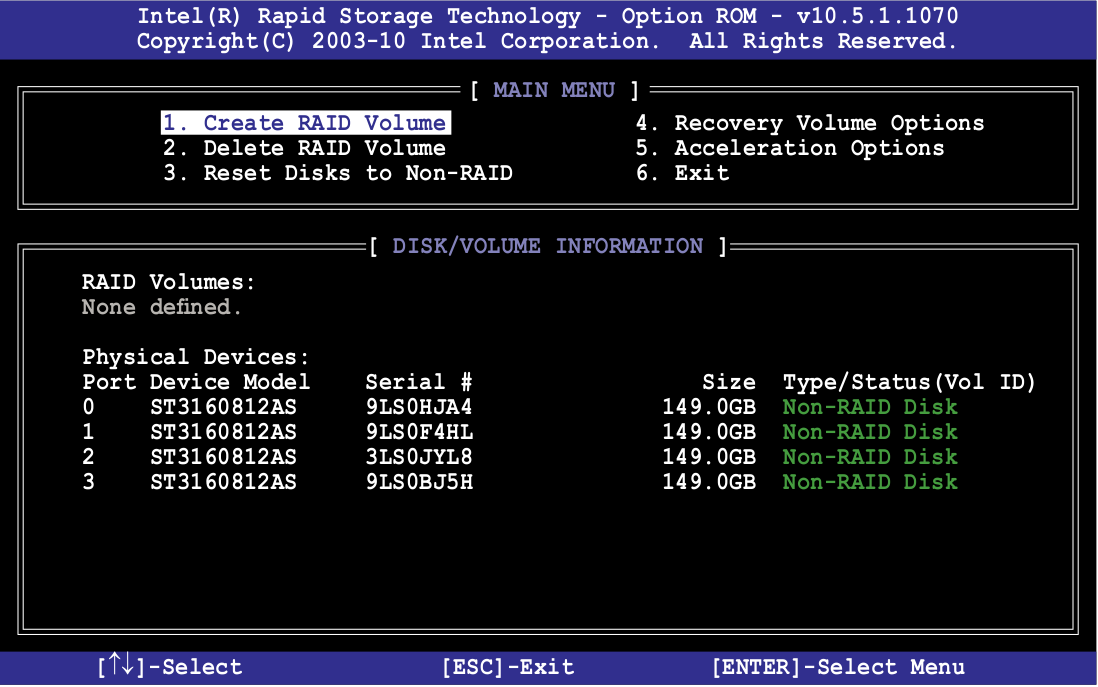
\includegraphics[width=0.4\textwidth]{raid}
\end{figure}
\item 创建RAID,选择Create RAID Volume。
\begin{figure}[!ht]
\centering
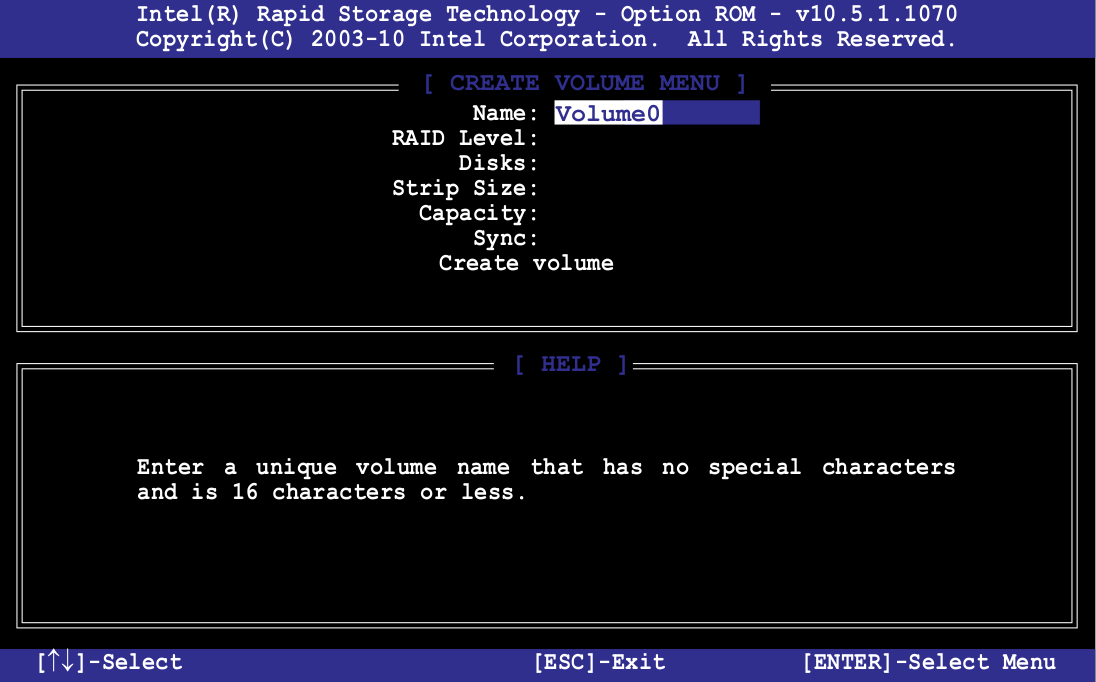
\includegraphics[width=0.4\textwidth]{creat_raid}
\end{figure}
\item 设置RAID,选中上图的选项中的Disks,显示下图。选择硬盘创建RAID。
\begin{figure}[!ht]
\centering
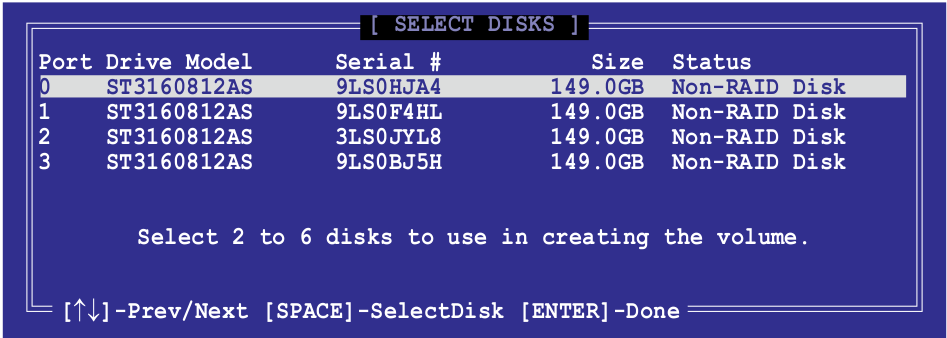
\includegraphics[width=0.4\textwidth]{select_raid}
\end{figure}
\item 创建成功的RAID,如图。RAID的status比较重要,应为Normal,如果出现Rebuild、Degrade、Failed等,请重新创建。
\begin{figure}[!ht]
\centering
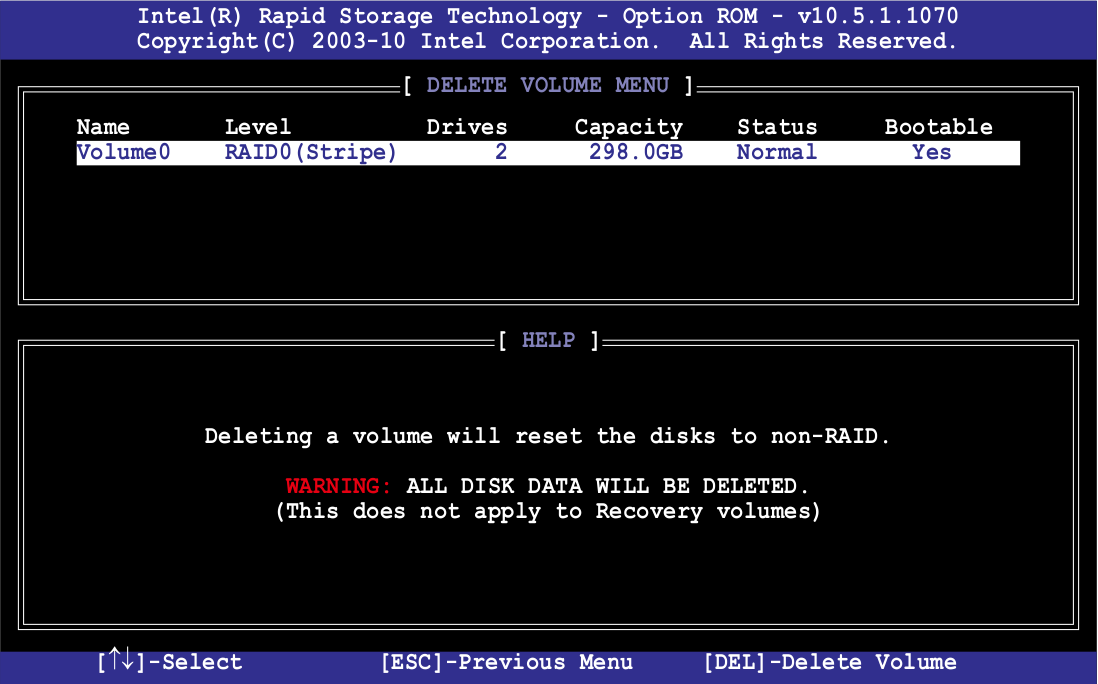
\includegraphics[width=0.4\textwidth]{delete_raid}
\end{figure}
\item 格式化,进入Ubuntu系统后,在/dev/mapper/下可看到RAID5被映射成为isw\_dfafd\_Volume1。将其格式化为Ext4文件系统。(对于大容量的硬盘的识别会出现问题,会显得比理论容量小;在Window系统下,不会出现这中情况。)
\begin{bash}
sudo mkfs.ext4 /dev/mapper/isw_dfafd_Volume1
\end{bash}
\item 挂载,将格式化好的映射硬盘,挂载到/deep目录下。
\begin{bash}
sudo mkdir /deep
sudo /dev/mapper/isw_dfafd_Volume1 /deep
\end{bash}
\item 自动挂载,为了重启后,直接使用映射硬盘,让其自动挂载。按照格式进入/etc/fstab
\begin{bash}
sudo vim /etc/fstab
\end{bash}
\end{enumerate}

\subsection{RAID5实验情况}
DIGITS DevBox的RAID5在各种软件配置和系统下的测试。目前X99主板集成的RAID功能,为Intel Rapid Storage Technology,在Linux下主要使用的是DM RAID和MD RAID,即dmraid和mdadm命令。DM RAID (dmraid)默认情况下,Ubuntu可以识别,但是已经几年没更新了;而mdadm经过几年的测试,在工业界更受欢迎。mdadm在Window下有UI界面,在Linux下只有命令行,其产生的中间数据支持两个系统下,可用在双系统环境下。在单Linux系统下,使用mdadm比较合适。

本此实验是使用3块3.6TB的硬盘,在BIOS中和Ubuntu系统下分别创建RAID5进行实验,理论上RAID5应该为7.2TB。
\begin{itemize}
\item 默认情况下,BIOS中已创建RAID5
	\begin{itemize}
	\item Ubuntu识别/dev/mapper/isw\_dafadfadsf\_Volume1,只有3.6TB 
	\item Ubuntu server无法用dmraid激活mapper,无法显示
	\item Debian不识别
	\end{itemize}
\item 安装mdadm的情况下,BIOS中已创建RAID5,但是ubuntu系统下mdadm不创建RAID5
	\begin{itemize}
	\item Ubuntu识别/dev/mapper/isw\_dafadfadsf\_Volume1,只有3.6TB 
	\item Ubuntu server无法用dmraid激活mapper,所以无法显示
	\item Debian不识别
	\end{itemize}
\item 安装mdadm和dmraid的情况下,BIOS中不创建RAID5,Ubuntu系统下mdadm创建RAID5
	\begin{itemize}
	\item Ubuntu不识别RAID5
	\item Ubuntu server识别RAID5为7.2TB
	\item Debian识别RAID5为7.2TB
	\end{itemize}
\end{itemize}
由以上实验,可以看出Ubuntu只识别dmraid所创建的RAID5的映像,而Ubuntu server和Debian都不能识别;对于mdadm所创建的RAID5,Ubuntu server和Debian在安装系统时,都能够识别,而Ubuntu不能够识别。

因此,考虑到目前的系统为Ubuntu14.04,而且需要使用硬盘的RAID5功能,且mdadm比dmraid更稳定与安全,所以在此决定使用mdadm创建软RAID。
%%---------------------------------------------------------------------
\end{document}
